\documentclass[11pt]{article}
\usepackage{natbib}
\usepackage{url}
\usepackage{graphicx}
\usepackage[acronym]{glossaries}


\newacronym{rmse}{RMSE}{Root Mean Square Error}
\newcommand{\rmse}{\gls{rmse}}



\newcommand{\myquote}[1]{\textit{#1}}
\newcommand{\fg}[1]{\citet{Annand2020}, fig. #1}

\newcommand{\xt}{x_{T}}
\newcommand{\yt}{y_{T}}

\newcommand{\xti}{x_{T,i}}
\newcommand{\yti}{y_{T,i}}

\newcommand{\xto}{x_{T,p}}
\newcommand{\yto}{y_{T,p}}

\newcommand{\target}{$\xt$ and $\yt$}
\newcommand{\nnin}{$\xti$ and $\yti$}
\newcommand{\nnout}{$\xto$ and $\yto$}

%opening
\title{Computational analysis of the Etch-A-Sketch task:\\ a commentary on Annand et al. (2020)}
\author{}

\begin{document}

\maketitle

%\begin{abstract}
%\end{abstract}

\citet{Annand2020} presented participants with a novel task setup. Their apparatus consists of a stylus on a computer screen controlled by two rotary dials. One dial controlled the stylys' movement in the $x$-direction while the other dial was used to control the $y$-direction. In this, the setup is reminiscent of \textit{Etch-A-Sketch}, the famous mechanical drawing device \citep{EtchASketch}. Using this apparatus, participants were instructed to trace a circle on the computer screen indicated by a thin black line. The target angular frequency was set by a moving target indicator overlaid on the circle. The indicator moved along the circular path with a period of either $\sim$5 seconds or  $\sim$2.5 seconds. Participants were instructed to \myquote{to match the position of their stylus with that of the target}.

Participants' performance in following the target indicator was evaluated as a function of the trial number. \citet{Annand2020} had both individual participants and dyads performing the task. When individuals performed the task, participants controlled both dials. Dyads controlled one dial each.

\citet{Annand2020} presented hypotheses about differences in the performance of dyads and individuals as a function of practice. However, we suggest that they did not test each of their hypotheses. Moreover, we conjecture that the analyses they do present are flawed. As the authors conclude that their setup can be \myquote{adapted to probe many different hypotheses of interlimb coordination and motor learning}, we think it is essential to provide a critique of the analyses presented and suggest additional and alternative data processing approaches. This would increase future researchers' ability to draw correct inferences from the data collected using this task and assess whether the setup is suitable to address their research question(s). 

The authors postulate three hypotheses.

\begin{itemize}
	\item{Hypothesis 1.} Individual participants start the training with inherently stable relative phase differences between limbs, particularly 0 or 180 degrees. Learning the required 90-degree phase difference requires practice.
	\item{Hypothesis 2.} The limbs of dyads are less strongly coupled than those of individuals.
	\item{Hypothesis 3.} From hypotheses 1 and 2, \citet{Annand2020} deduced a third hypothesis: performance of individuals would be initially worse. Still, it should exceed dyads' performance after training because individuals can attain stronger 90-degree shift coupling.
\end{itemize}

\section{Testing hypothesis 1}

\citet{Annand2020} do not attempt to test hypothesis 1. In a footnote, the authors suggest that the phase shift between the limbs can not be assessed because their traces are not strictly sinusoidal. They state that they \myquote{were unable to utilize explicitly phase-based measures of performance, as participants' movements, specifically during early trials when they were still exploring the task-space, were not always oscillatory.} However, we suggest the data allows assessing the phase relationship between limbs, both within and across trials. In turn, this allows testing one of the hypotheses that leads them to propose hypothesis 3. 

\begin{figure*}[htb]
	\centering
	\includegraphics[width=1\linewidth]{images/trial_1.pdf}
	\caption{Analysis of trial 1 (Data from \fg{5}). (a) The $x_t$ and $y_t$ traces. (b,c) The magnitude spectra of $x_t$ and $y_t$. The red line indicates the target frequency set by \citet{Annand2020}. (d) The frequency-average phase shift as a function of time. The horizontal lines indicate 180 and 90 degree phase shifts.}
	\label{fig:trial1}
\end{figure*}


To test hypothesis 1, we need to evaluate the phase shift between $x_t$ and $x_t$. We propose calculating the complex spectrogram of $x_t$ and $y_t$ using a window covering several periods of the target signal. Next, we extract the phases from each spectrogram for the frequency channels with at least 10\% of the energy of the frequency channel with the most energy. We take the difference between the selected channels for $x_t$ and the selected channels for $y_t$. Finally, we average across the frequency channels. This operation results in the phase difference between $x_t$ and $y_t$, as a function of time, averaged across the most prominent frequency channels.

We find that the phase difference between $x_t$ and $x_t$ is 90 degrees from the start of the training (i.e.,  trial 1). There is little or no evidence in the reported data that phase offsets between limbs shifts from 0 or 180 to 90 degrees. 

In figure \ref{fig:trial1}, we show the result of the analysis for trials 1 (data from \fg{5}). In this early training trial, $x_t$ and $y_t$ have a 90 degrees phase relationship throughout the trial. The angular relationship between $x_t$ and $y_t$ is somewhat more variable than later in the training (see figs. \ref{fig:trial5}, \ref{fig:trial10}, \ref{fig:trial15}, \ref{fig:trial20}).


It should be noted that figure \ref{fig:trial1} reveals that it is mainly the low frequency of the $x_t$ and $y_t$ motions in trial 1 that drive the larger \rmse: the period of the participant's motion is about 10 sec in trial 1 instead of the 5-sec target speed. We also analyzed the data for trials 5, 10, and 20 (\fg{5}). In all cases, we found a nearly constant phase relationship of  90 degrees between the $x_t$ and $y_t$ (see figs. \ref{fig:trial5}, \ref{fig:trial10}, \ref{fig:trial15}, \ref{fig:trial20}).



\citet{Annand2020} depict data for an individual and a dyad who \myquote{failed to produce stable coordination with the target by the end of the experiment} (\fg{7}). Analyzing these data, we found that these participants also attained a 90-degree phase shift (figs. \ref{fig:ind} and \ref{fig:dyad}). However, in both cases, the participants' motions were slightly too slow (compared with the required target speeds). This resulted in large \rmse\ values.

Finally, we reanalyzed the data for the participant in the \myquote{exploration stage} \fg{4} (see fig. \ref{fig:explore}). We did not find strong evidence for an initial 180/0 degree phase relationship even for these data. There are some parts of the trial where the participant seems to have a 180-degree shift between the limbs. However, mostly, the shift hovers around 90 degrees. 

We conclude that the data shown by \citep{Annand2020} do not provide evidence of an initial 180/0 degree phase relationship between limbs that needs to be unlearned throughout the training. In contrast, the data provided in their paper suggests that participants mainly learned to execute the motions fast enough and that the \rmse\ measure predominantly picks up differences between the required and the actual speed of the participants. 

We also conclude that, in contrast to the author's assertion that the participant's trajectory in trial 1 was \myquote{aperiodic} (data depicted in \ref{fig:trial1}), spectral analysis shows a strong periodicity in this signal (i.e., with a frequency of about 0.1 Hz).

The finding that participants did not start out using a 0/180 degree phase shift despite \citet{Annand2020} citing considerable evidence to leading them to expect this made us to question whether the task precluded this from happening. We conjecture that the setup biased participants to adopt a 90 degree phase shift. Indeed, \citet{Annand2020} did not only show participants a target that followed a circular trajectory. Throughout the experiments, \myquote{the circle that the target traced was also continuously indicated on the screen in a thin, black line}. Therefore, at any point in time, the participants could have moved the dials such that their cursor coincided with this target circle. Aiming the cursor to coincide with the circle \textit{ipso facto} leads to a 90 degree phase shift between the $x$ and $y$ trajectories. In other words, the visible circle provided participants direct and continuous feedback enabling them to maintain a 90 degree phase shift between $x_t$ and $y_t$. 

\section{Testing hypothesis 2}

The authors presumed, based cited evidence, that the dyads are \myquote{relatively weaker coupled than the limbs of the individuals}. However, they do not assess whether their data supports this conjecture. 

Testing hypothesis 2 is problematic for two reasons. First, the authors provide very little data that would allow assessing whether dyads have a weaker intrinsic coupling. They only provide one trace of a dyad they labeled as uncoordinated \fg{7}. The authors can address this issue as they have access to the full data set. A second, more theoretical, problem is that the authors do not specify what kind of coupling they expect between the limbs of individuals or dyads. In the absence of a model of the expected coupling, it is difficult to assess its strength.

Nevertheless, we attempted to assess differences in coupling strength across the trials \fg{5} and compare this with the data for the single dyad \fg{7}. To do so, we need to postulate a definition of coupling. One plausible (and simple) definition could a correlation of the behavior for the left and the right hand (or the two people in a dyad).

Under this definition, we could correlate the phase and magnitude spectra of the $x_t$ and $y_t$ traces to assess coupling strength. Doing so shows that coupling strength is high (correlation close to 1) across trials (fig. \ref{fig:strength}). The data for the single dyad shown by \citep{Annand2020} has comparable coupling strength, even though the authors labeled these participants as being unable to attain coordination. The dyad's coupling seems to be stronger than for the initial stages of the individual's training depicted (\fg{5}) and participant in the exploration phase (\fg{4}).

\begin{figure}[t]
	\centering
	\includegraphics[width=0.5\linewidth]{images/strength.pdf}
	\caption{Assessment of the coupling strength between the limbs of individuals and the two participants in a dyad. As \citet{Annand2020} do not provide a definition of coupling, we postulate that correlation between $x_t$ and $y_t$ can be used to quantify coupling. This graph shows the Pearson correlation of the phase and magnitude spectrogram of $x_t$ and $y_t$ for all data presented by \citet{Annand2020}. Black lines: data from \fg{5}, Green and Red: data from \fg{7}. Blue: data from \fg{4}. Round markers: correlation of the amplitude spectrogram. Square markers: correlation of the phase spectrogram.}
	\label{fig:strength}
\end{figure}

We conclude that, based on the very limited data provided by \citet{Annand2020} and our proposed definition of coupling, there is no evidence to support the assertion that the dyads are relatively weaker coupled.

\section{On the use of \rmse}

\citet{Annand2020} rely on \rmse\ measures to test hypothesis 3. Obviously, \rmse\ can be used as a measure of task performance. However, here we argue that analysis of the performance on the task (as measured by \rmse\ or another error measure) is not suited to draw inference about coupling between limbs or dyads. \rmse\, or any other measure of task performance, can not be used to draw conclusions about physical or functional coupling.

Using a generative model, we show that the $x$-component of the task can be solved independently from the $y$ component of the task. We use a fully connected feedforward neural network without hidden layers. We train the network to take 15 samples of the $\xt$ and $\yt$ target positions and generate the next 15 samples. In other words, we train the neural network to predict the future positions (\nnout) of the target on the computer screen from a sequence of past positions (\nnin). We train the network using 500 examples, which random phase offsets.

Figure \ref{fig:coupled}a shows (for a single example input) that the network can predict the future position of the target (\nnout) based on past samples (\nnin). Figure \ref{fig:coupled}b,c show that the training algorithm has found a solution that results in some coupling between how the outputs \nnout\ are generated. Replacing the input for $x$ ($\xti$) with noise disrupts the predictions for both $\xto$ and $\yto$ (Figure \ref{fig:coupled}b). The symmetrical result occurs when $\yti$ is replaced with noise  (Figure \ref{fig:coupled}c). This implies the outputs \nnout\ are coupled to the same generative process. Indeed, this can be inferred from inspecting the neural network's weight matrix. Each output unit takes input from both input units coding for  $\xti$  and $\yti$ . In summary, figure \ref{fig:coupled} shows that the task can be solved using an algorithm that introduces some dependency (in the generation of) the outputs \nnout.

We can also train the network without introducing dependency between the generation of \nnout. In figure \ref{fig:uncoupled} we show the results for a network trained with constraints on the weight matrix. In particular, we clamped all connection between  $\xti$ ($\yti$) and $\yto$ ($\xto$) to zero. Essentially, this results two idependent neural networks that learn to predict $\xto$ soley based on $\xti$ and  $\yto$ soley based on $\yti$. The network still learns to predict \nnout. This results shows that the task used by \citet{Annand2020} consists of two independent subtasks that can be solved without any coupling between the processes solving each component.

\begin{figure*}[t]
	\centering
	\includegraphics[width=1\linewidth]{images/uncoupled.pdf}
	\caption{Results of training a feedforward neural network to predict the next 15 samples the target signals \target\ (\nnout) based on the 15 past samples (\nnin). In these results, the networks connection matrix was constrained. (a) A single example of inputs \nnin (full lines) and the predicted subsequent samples, \nnout (dashed lines). The thick gray lines show the target values for \nnout. (b) Similar as for panel (a) but $\xti$ was replaced with a noise signal. (c) Similar as for panel (a) but $\yti$ was replaced with a noise signal. (d) The weight matrix of the trained neural network.}
	\label{fig:uncoupled}
\end{figure*}

Our modeling exercise present a computational analysis that reveals different algorithmic solutions to the same task \citep{Marr2010}. Indeed, the modeling results show that the task allows participants to attain perfect performance (\rmse\ $\sim$ 0) by either coupling the motion of the left hand to the right or by controlling each limb independently. As such, the \rmse\ values can not be used to evaluate hypothesis 1 and hypothesis 2. Moreover, as differences in the underlying functional coupling do not necessarily lead to differences in \rmse, no prediction can be made about the relative performance of participants based on assumptions about coupling strengths. Therefore, hypothesis 3 can not be tested using \rmse\ values, nor can valid predictions be made from the assumptions about the evolution of the \rmse. The over-reliance of the authors on the \rmse\ is also shown by the implications they ascribe to decreasing \rmse. They state that,

\vspace{11pt}
\noindent \myquote {[a] reduction in [\rmse] indicates, ipso facto, the following changes in coordination between the two dials: 1) convergence toward  $\phi = 90^\circ$, 2) reduced variability about $\phi = 90^\circ$, 3) proper movement amplitude, and 4) better coordination in time with the target.}
\vspace{11pt}

This statement is not true. A \textit{decrease} in \rmse\ does not \textit{ipso facto} lead to these 4 outcomes. We agree that for \rmse\ $=0$, participants' traces would perfectly match the targets \target\ in amplitude, phase and frequency. However, as long as \rmse\ $>0$, the conjecture of the authors does not hold. 

Concerning points 1 and 2, we show that the phase offset is 90 degrees throughout the training while the \rmse\ decreases (\fg{5}). In fact, we show that the decrease in \rmse\ is mostly driven by the participants attaining the target frequency and not the target phase offset (See figures \ref{fig:trial1}, \ref{fig:trial5}, \ref{fig:trial10}, \ref{fig:trial15}, \ref{fig:trial20}). Therefore, the \textit{decrease} in \rmse\ observed by \citet{Annand2020} does not necessarily imply a convergence to a 90 degree phase shift.

Concerning point 3, a decrease in \rmse\  does not necessarily imply that the movement amplitude converges to 1. Again, this can be seen in the data (\fg{5}): the amplitude of the motions does not change as a function of training. Yet, the \rmse\ decreases monotonically. Again, the  observed decrease in \rmse\ is mostly driven by frequency matching. Not, amplitude matching.

Finally, concerning point 4, the authors do not provide a definition of \textit{good coordination}. In absence of such a definition it is possible to argue that coordination is can attained with large \rmse\ values. For example, the participants could generate $x$ and $y$ traces in perfect anti-phase with the target $\xt$ and $\yt$. In this case, the participant would, arguably, be in good coordination but generate high \rmse\ values.

In their conclusion, \citet{Annand2020} state that their study \myquote{[shows that] interlimb coordination is
 differentially constrained for intra-or interpersonal coupling} and that 
\myquote{[this was caused by] differential interference
from intrinsic coordination dynamics arising from differences in coupling strength.} As stated above, \citet{Annand2020} fail to test these hypotheses, which our analyses failed to support. Moreover, in this section, we show that \rmse\ can not be used to test assertions about coupling in this task. It is simply not a good enough measure. 

\section{Conclusion}

\citet{Annand2020} postulate two hypotheses about the coupling between limbs and dyads. Neither of these where tested by \citet{Annand2020}. Reavaluting the provided data, we found no evidence supporting them. We conjecture this is at least partly caused by the continuous, direct feedback provided in the form of a circle on the screen. This provided  participants with a means to easily adopt a 90 degree phase offset.

Moreover, we show, using a generative model, that inferences about coupling solely based on \rmse\ are flawed. Low \rmse\ values can be obtained without any functional coupling between the limbs or dyads. In addition,  \rmse\ is simply not a good enough measure to understand the behavior of participants in this task.

By suggesting (1) additional analysis methods, (2) pointing out a potential issue with the experimental task, and (3) warning about the use of \rmse, we hope to benefit researchers who wish to \myquote{[adapt this task] to probe many different hypotheses of interlimb coordination and motor learning}.

\bibliographystyle{plainnat}
\bibliography{refs}

\setcounter{figure}{0} 
\appendix
\renewcommand\thefigure{S\arabic{figure}}
    
\section*{Supporting material}


\begin{figure*}[htb]
	\centering
	\includegraphics[width=1\linewidth]{images/trial_20.pdf}
	\caption{Analysis of trial 5 (Data from \fg{5}). Similar as figure \ref{fig:trial1}}
	\label{fig:trial5}
\end{figure*}


\begin{figure*}[htb]
	\centering
	\includegraphics[width=1\linewidth]{images/trial_10.pdf}
	\caption{Analysis of trial 10 (Data from \fg{5}). Similar as figure \ref{fig:trial1}}
	\label{fig:trial10}
\end{figure*}



\begin{figure*}[htb]
	\centering
	\includegraphics[width=1\linewidth]{images/trial_15.pdf}
	\caption{Analysis of trial 15 (Data from \fg{5}). Similar as figure \ref{fig:trial1}}
	\label{fig:trial15}
\end{figure*}

\begin{figure*}[htb]
	\centering
	\includegraphics[width=1\linewidth]{images/trial_20.pdf}
	\caption{Analysis Trial 20 (Data from \fg{5}). Similar as figure \ref{fig:trial1}}
	\label{fig:trial20}
\end{figure*}

\begin{figure*}[htb]
	\centering
	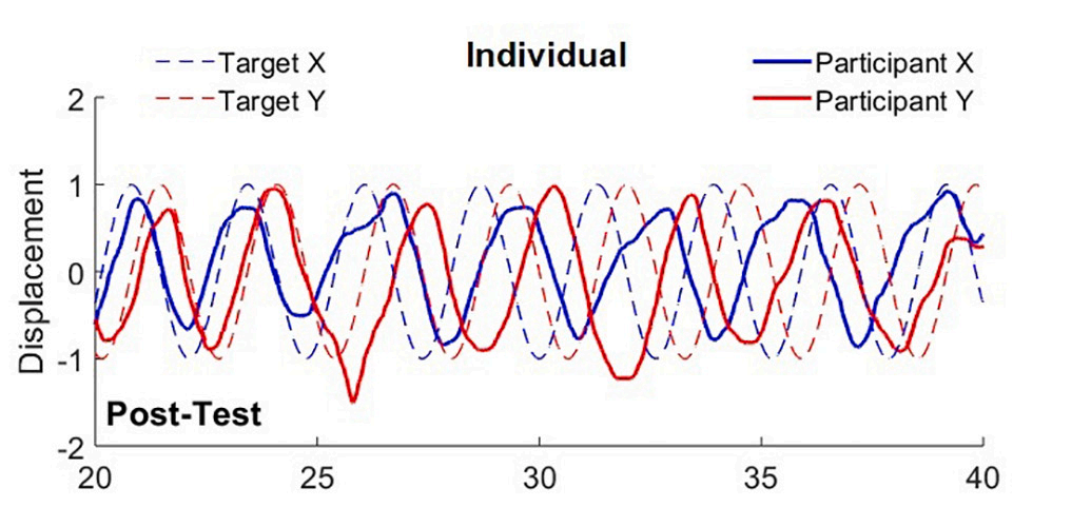
\includegraphics[width=1\linewidth]{images/ind.pdf}
	\caption{Analysis of the data of the individual that \myquote{failed to produce stable coordination with the target by the end of the experiment} (\fg{7}). Similar as figure \ref{fig:trial1}}
	\label{fig:ind}
\end{figure*}


\begin{figure*}[htb]
	\centering
	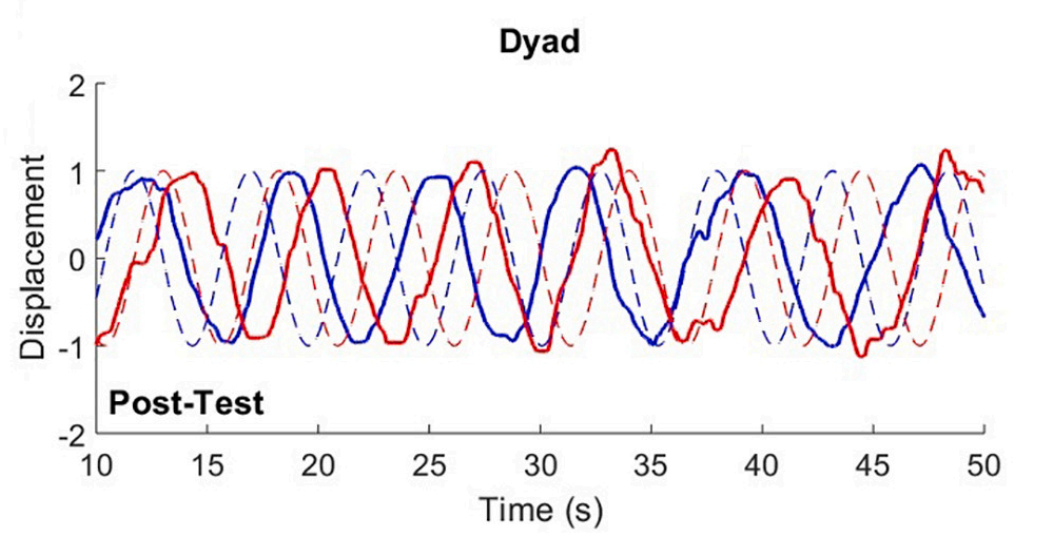
\includegraphics[width=1\linewidth]{images/dyad.pdf}
	\caption{Analysis of the data of the dyad that \myquote{failed to produce stable coordination with the target by the end of the experiment} (\fg{7}). Similar as figure \ref{fig:trial1}}
	\label{fig:dyad}
\end{figure*}


\begin{figure*}[htb]
	\centering
	\includegraphics[width=1\linewidth]{images/explore.pdf}
	\caption{Analysis of the data of a participant in the \myquote{exploration stage} (\fg{4}). Similar as figure \ref{fig:trial1}}
	\label{fig:explore}
\end{figure*}



\begin{figure*}[htb]
	\centering
	\includegraphics[width=1\linewidth]{images/coupled.pdf}
	\caption{Results of training a feedforward neural network to predict the next 15 samples the target signals \target\ (\nnout) based on the 15 past samples (\nnin). (a) A single example of inputs \nnin (full lines) and the predicted subsequent samples, \nnout (dashed lines). The thick gray lines show the target values for \nnout. (b) Similar as for panel (a) but $\xti$ was replaced with a noise signal. (c) Similar as for panel (a) but $\yti$ was replaced with a noise signal. (d) The weight matrix of the trained neural network.}
	\label{fig:coupled}
\end{figure*}








\end{document}
